% Chapter: Methods (porous reframe)

\section{Overview}
\label{sec:meth_overview}

The methodology follows a characterise-before-train philosophy: before asking how a structured excitable medium might be optimised for a computational task, we first measure, in a controlled and reproducible way, what the unoptimised medium already does.
It has four layers.

The model layer describes the BZ medium by the two-variable Tyson--Fife Oregonator, extended with substrate knobs that act as candidate weights: wall geometry, a light-suppression field, and an anisotropic diffusion tensor.
The solver layer is an explicit finite-difference scheme with adaptive reaction subcycling, verified against known excitable-media phenomenology and convergence-tested in space and time.
The protocol layer is a black-box characterisation: the substrate is stimulated at defined input ports and its response recorded at fixed probes, yielding transfer functions rather than snapshots.
The composition layer translates the measured transfer functions into an event-driven graph simulator and validates it against full PDE solutions.

\section{The Oregonator Model}
\label{sec:meth_oregonator}

\subsection{Two-Variable Reduction}
\label{sec:meth_oregonator_2var}

The chemical basis of the substrate is the BZ reaction, modelled by the two-variable Tyson--Fife reduction of the Oregonator introduced in \refSec{sec:lit_bz} \cite{field1974oregonator, tyson1980target}.
In the scaled Tyson--Fife form used throughout this thesis, the kinetics are
\begin{equation}
\frac{\partial u}{\partial t} = \frac{1}{\varepsilon}\left[\,u - u^{2} - \left(f v + \phi\right)\frac{u - q}{u + q}\,\right] + \nabla\!\cdot\!\left(\mathbf{D}\,\nabla u\right),
\label{eq:oregonator_u}
\end{equation}
\begin{equation}
\frac{\partial v}{\partial t} = u - v + D_{v}\,\nabla^{2} v,
\label{eq:oregonator_v}
\end{equation}
where $u$ is the scaled activator concentration, $v$ the scaled oxidised catalyst concentration, and $\phi$ the illumination in the photosensitive ruthenium-catalysed variant \cite{sakurai2002design}.
The parameter $\varepsilon \ll 1$ sets the timescale separation, $f$ is a stoichiometric factor, and $q \ll 1$ is a scaling ratio.
This singularly perturbed structure gives the medium its excitable pulse dynamics \cite{tyson1988singular}.

The Barkley model \cite{barkley1991model} is retained as a phenomenological cross-check:
\begin{equation}
\frac{\partial u}{\partial t} = \frac{1}{\varepsilon}\,u\left(1 - u\right)\left(u - \frac{v + b}{a}\right) + D_{u}\,\nabla^{2}u,
\qquad
\frac{\partial v}{\partial t} = u - v.
\label{eq:barkley}
\end{equation}
Its polynomial nonlinearity removes the stiffness of the Oregonator rational term, making it a fast workhorse; headline results are cross-checked against the chemically grounded Oregonator.

\subsection{Physical Units and Scaling}
\label{sec:meth_scaling}

The dimensionless variables are rescalings of physical concentrations \cite{tyson1980target}:
\begin{equation}
u = \frac{2 k_{4}}{k_{3} A}\,[\mathrm{HBrO_{2}}],
\qquad
v = \frac{k_{c} k_{4} B}{(k_{3} A)^{2}}\,[\mathrm{Ce(IV)}],
\qquad
\tau = k_{c} B\,t,
\label{eq:tyson_fife_scaling}
\end{equation}
where $t$ is physical time and $A$, $B$ are bath-species concentrations.
With reference values $A = 0.06$ M, $B = 0.02$ M, one model time unit corresponds to about 50 s and one grid cell to about 0.3 mm \cite{field1986oxybromine}.
The measured model pulse speed of 6.2 cells per time unit maps to about 0.04 mm/s, within a factor of about four of the 0.15 to 0.2 mm/s reported for photosensitive BZ layers \cite{suematsu2021instability}, the level of agreement expected given recipe dependence.
This mapping is a calibration, not an identity; the simulations use the computational parameter set $\varepsilon = 0.05$, $q = 0.002$, $f = 1.4$, standard in the wave-simulation literature.

\subsection{Reaction-Diffusion Formulation}
\label{sec:meth_rd}

The activator diffuses with coefficient $D_{u}$ (generalised to a tensor in \refSec{sec:meth_anisotropy}), while the recovery variable is taken as immobile, $D_{v} = 0$.
Channel walls and domain boundaries impose no-flux (homogeneous Neumann) conditions, enforced by zeroing diffusive fluxes on wall-adjacent faces.
All simulations use the model's nondimensional units: space in grid cells, time in model time units, speeds in cells per time unit.

\section{Regime Identification}
\label{sec:meth_regime}

The BZ reaction is oscillatory by default, but pulse computation requires an excitable regime in which the rest state is stable.
A linear-stability scan of the Oregonator rest state over the $(\varepsilon, \phi)$ plane shows that the baseline parameters $f = 1.4$, $\varepsilon = 0.05$, $q = 0.002$, $\phi = 0$ give an unstable node; raising the background illumination stabilises the rest state.
At the adjusted stoichiometric factor $f = 1.4375$, illumination levels $\phi \geq 0.01$ yield a stable excitable regime.

The working point used for all measurements in this thesis is candidate A: $\varepsilon = 0.0501$, $\phi = 0.010$, with rest state $u^{*} = v^{*} = 0.00308$ and stable eigenvalues.
A second working point, candidate B ($\varepsilon = 0.0199$, $\phi = 0.010$), supports faster pulses and pairs naturally with the Barkley kinetics.

A finer sweep of $\phi$ at $\varepsilon = 0.0501$ distinguishes three regimes.
For $\phi \lesssim 0.0045$ the rest state is unstable and the medium oscillates.
For $0.0045 \lesssim \phi \lesssim 0.026$ the medium is excitable and supports propagating pulses.
For $\phi \gtrsim 0.026$ the rest state is stable but a launched pulse attenuates before travelling far.
The usable computing window is therefore
\begin{equation}
0.005 \lesssim \phi \lesssim 0.026,
\label{eq:phi_window}
\end{equation}
and the working point $\phi = 0.010$ lies near its centre.

\begin{figure}[htbp]
\centering
\IfFileExists{../Analysis/figures/pub/pub_regime_map.png}{%
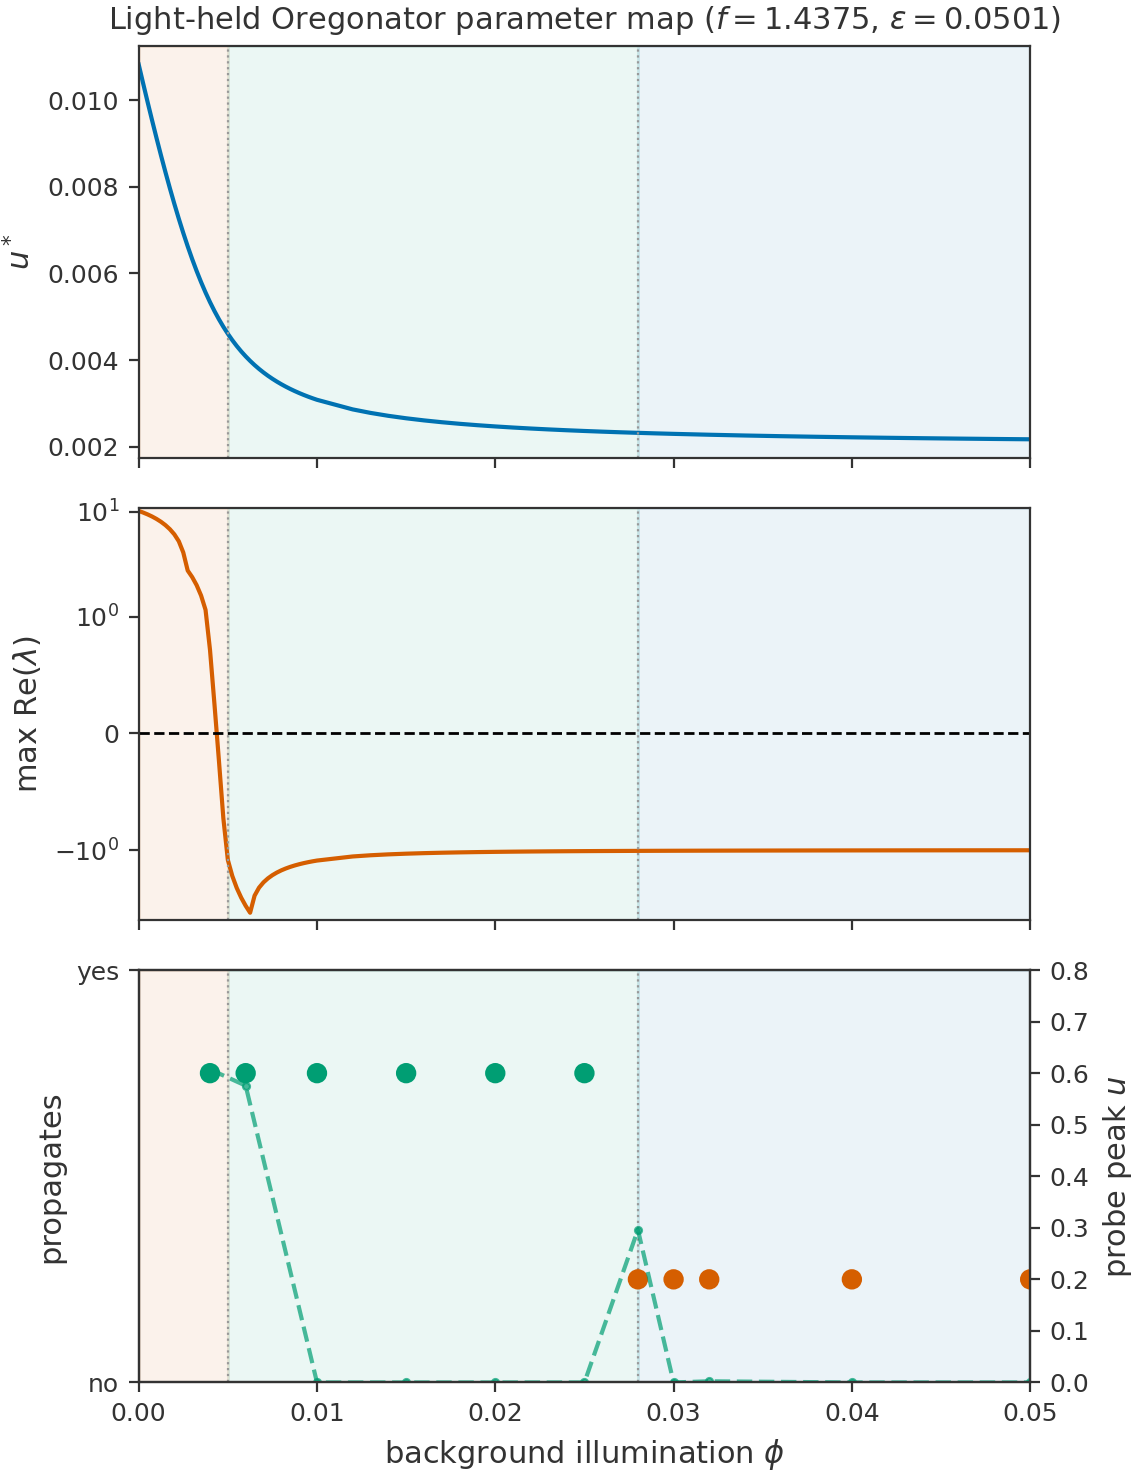
\includegraphics[width=0.85\textwidth]{../Analysis/figures/pub/pub_regime_map.png}}{%
[figure pending]}
\caption{Oregonator regime map in the $(\varepsilon, \phi)$ plane. The excitable propagation band lies between the oscillatory and attenuated regimes; the working point is marked near the centre of the band.}
\label{fig:meth_regime}
\end{figure}

\section{Numerical Solver and Verification}
\label{sec:meth_solver}

\subsection{Discretisation}
\label{sec:meth_discretisation}

The equations are discretised on a regular two-dimensional Cartesian grid with spacing $\Delta x = 1$ cell and time step $\Delta t = 0.05$ time units.
The diffusion term is discretised in divergence (flux) form, with face-averaged tensors and central differences, reducing to the standard five-point Laplacian when the tensor is isotropic.
No-flux walls are enforced at the flux level by zeroing fluxes on wall-adjacent faces.
The explicit diffusion stability constraint $D\,\Delta t / \Delta x^{2} \leq 1/4$ is satisfied at the working resolution.

The fast activator kinetics are stiff, so time integration uses first-order operator splitting with adaptive reaction subcycling.
Within each outer step the reaction substep $h$ is chosen from the analytic Jacobian: $h \leq 0.5 / \max(-\partial F/\partial u,\,0)$.
A relative-accuracy limit and an absolute step-size limiter prevent $u$ from being pushed below $-q/2$ complete the rule.
A NaN/Inf tripwire aborts any run in which a field leaves the finite range.

\subsection{Verification Cases}
\label{sec:meth_verification}

The solver was verified against canonical excitable-media phenomenology: target waves, head-on collision and annihilation, gap diffraction, and timing control.
Grid refinement at $\Delta x = 1$, $0.5$, $0.25$ and timestep refinement about $\Delta t = 0.05$ were applied to the plane-pulse speed.
The full convergence study is reported in \refSec{sec:res_verification}; the spatial deficit is carried openly as an explicit error bar wherever absolute speeds are quoted.

\section{Substrate Parameterisation}
\label{sec:meth_parameterisation}

Three physically distinct parameterisations are used.

\subsection{Wall Geometry}
\label{sec:meth_walls}

Walls are a boolean mask; masked cells are impermeable and no-flux conditions are enforced at adjacent faces.
They define input ports, channels, and junctions.

\subsection{Light-Suppression Field}
\label{sec:meth_light}

The field $\phi(x,y)$ enters through the term $(f v + \phi)(u-q)/(u+q)$ in \refeqn{eq:oregonator_u}; locally increasing $\phi$ raises the effective threshold and suppresses excitability.
A uniform background value sets the operating regime; spatial modulation defines rewritable channels and barriers.

\subsection{Anisotropic Diffusion Tensor}
\label{sec:meth_anisotropy}

The activator diffusivity is replaced by a symmetric positive-definite tensor field $\mathbf{D}(x,y)$, parameterised by eigenvalues $D_{\parallel} \geq D_{\perp} > 0$ and fibre direction $\theta(x,y)$.
Eikonal theory predicts the pulse speed along the fast axis exceeds that along the slow axis by $\sqrt{r}$, where $r = D_{\parallel}/D_{\perp}$ \cite{keener1991eikonal}.

\section{Black-Box Characterisation Protocol}
\label{sec:meth_protocol}

All experiments share a black-box protocol.
Inputs are applied at ports: small circular regions where the light field is temporarily reduced to emit pulses.
Outputs are recorded at probes: fixed locations storing the mean activator value $u(t)$ over a small mask.
The internal state away from ports and probes is not inspected for a measurement; every result is an input-output transfer function.

The dark-spot drive is a one-shot flash of darkness: a circular patch is dimmed from $\phi = 0.010$ to $\phi = 0.002$ for a calibrated duration.
Flashes of $T_{\mathrm{flash}} \leq 4$ time units emit exactly one full-amplitude pulse; the operating point used here is $T_{\mathrm{flash}} = 3.0$ time units.

\begin{figure}[htbp]
\centering
\IfFileExists{../Analysis/figures/pub/pub_flash_calibration.png}{%
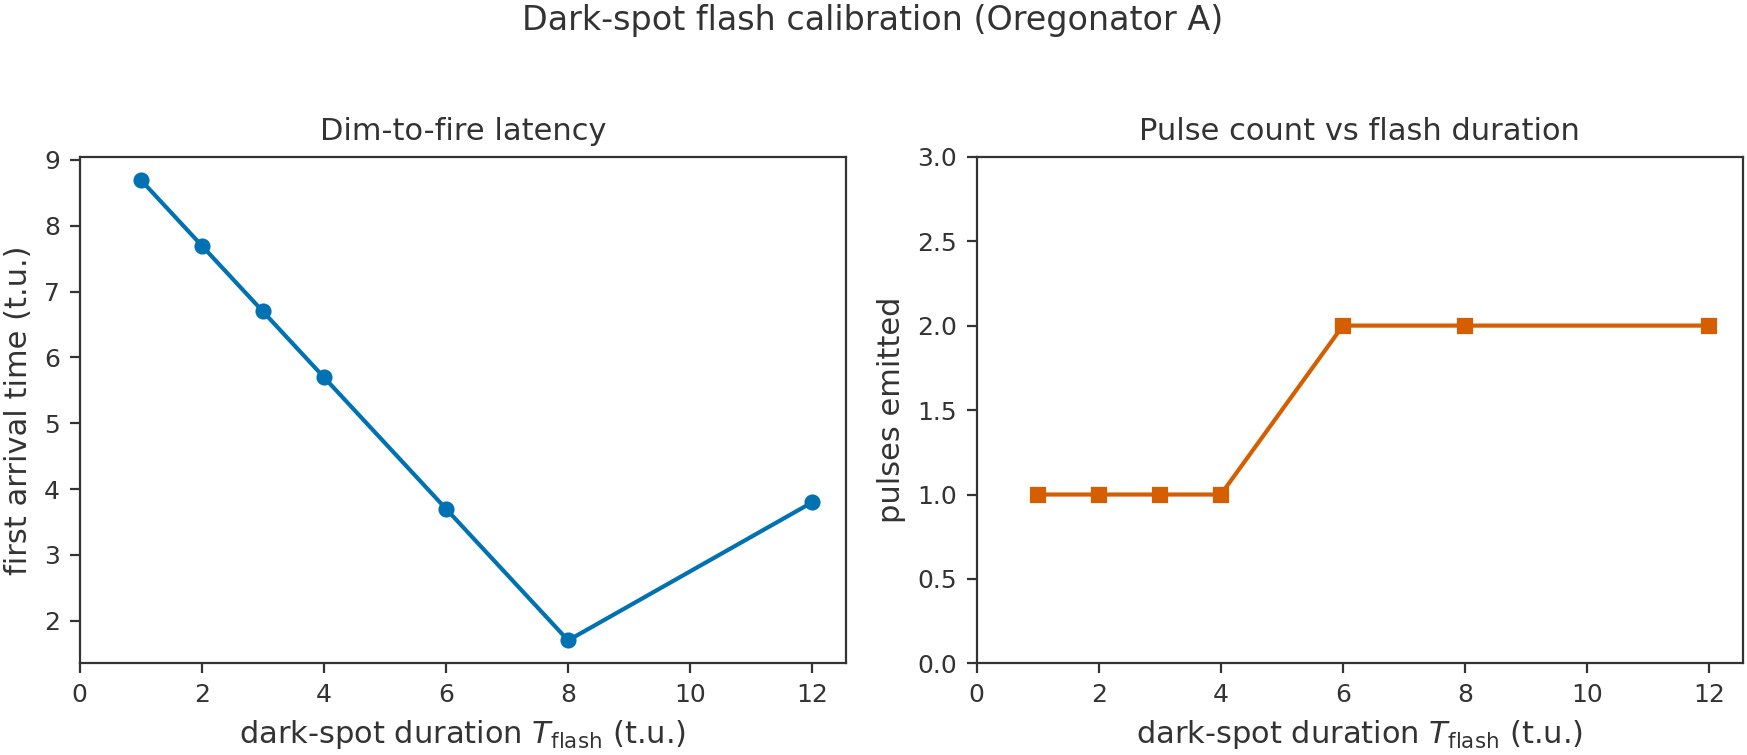
\includegraphics[width=0.85\textwidth]{../Analysis/figures/pub/pub_flash_calibration.png}}{%
[figure pending]}
\caption{Dark-spot flash calibration. Flash durations up to 4 time units emit a single pulse; longer flashes become sustained pacemakers. The operating point $T_{\mathrm{flash}} = 3.0$ time units is marked.}
\label{fig:meth_flash}
\end{figure}

Probe readouts are evaluated within defined time windows rather than over the whole record, because at an open junction a lone pulse diffracts into all connected branches and a whole-record readout would compute OR regardless of design intent.
The window is aligned to the expected collision outcome, isolating the annihilation event from the unconditional diffraction background.

\section{The Pore-Scale Experiments}
\label{sec:meth_experiments}

\subsection{Channel Pulse Transfer}
\label{sec:meth_exp_channel}

A straight channel of fixed width is cut between two walls, a single pulse is injected at the input port, and a far probe records the arrival.
Measured quantities: propagation speed, delay linearity, and transmission behaviour as width is swept.

\subsection{Frequency Response}
\label{sec:meth_exp_frequency}

A pulse train of prescribed frequency is injected and the probe records which pulses transmit.
Two forms: a two-pulse interval sweep locating the absolute refractory period, and a sustained-train measurement giving the maximum 1:1 following rate.

\subsection{Two-Input Inhibition}
\label{sec:meth_exp_logic}

Two input channels converge on a T-junction.
The four input combinations of a two-input truth table are applied; the probe record is converted into truth-table entries using the windowed readout.
Figures of merit: truth table, separation ratio, and inhibition window.

\subsection{Anisotropic Routing}
\label{sec:meth_exp_anisotropy}

In a uniform tensor field with anisotropy ratio $r$, a point stimulus is fired and the expanding pulse is tracked.
The $\sqrt{r}$ eikonal law provides a quantitative check, and a patch of anisotropic medium embedded in isotropic substrate measures orientation-dependent delay.

\section{Graph Simulator Construction}
\label{sec:meth_graph}

The measured transfer functions are translated into an event-driven graph simulator.
A node represents a pore or junction; an edge represents a throat.
Each edge carries a transit time $L/c$, where $L$ is the edge length in cells and $c$ is the measured pulse speed.
Each node carries a refractory time $\tau$, the interval after a pulse arrives during which the node ignores further pulses.
Each node also carries an inhibition window $w$: two pulses arriving at the same node within $w$ time units annihilate.
A routing table at each node decides which incoming edges feed which outgoing edges, encoding the junction topology.

The simulator processes pulses in order of arrival time.
When a pulse reaches a node, it is dropped if the node is refractory or if another pulse arrived within the inhibition window; otherwise it marks the node refractory and forwards copies to the allowed outgoing edges.
The simulator returns the arrival times and amplitudes at every probe.
It is fast enough to explore candidate networks in milliseconds, and its predictions are validated against PDE solutions in \refSec{sec:res_graph}.

\section{Three-Dimensional Extension}
\label{sec:meth_3d}

The graph simulator is dimensionless; the same nodes, edges, and rules apply in any dimension.
Extending the PDE solver to three dimensions requires a 7-point diffusion stencil, a 3D wall mask, and a 3D $\phi$ field.
The explicit stability limit becomes $D\,\Delta t / \Delta x^{2} \leq 1/6$.
Memory and compute grow as the cube of the linear domain size.

The practical blocker for full 3D pore networks is not the numerics but the light field: a projected 2D mask only controls the surface or a thin slab of a 3D bulk.
Without a known $\phi(x,y,z)$ in the interior, the local kinetics are uncontrolled.
The 3D results in \refSec{sec:res_3d} therefore use a thin-slab geometry and treat the extension as a boundary experiment rather than a validated network.
